%%%%%%%%%%%%%%%%%%%%%%%%
% GSL
%%%%%%%%%%%%%%%%%%%%%%%%

\subsubsection{Purpose}
\noindent \ac{EMTG} depends on \ac{GSL} for cubic-splining utilities. \\ \ac{EMTG} is known to work with \hl{GSL 2.4.0}. 

\subsubsection{Bundled Installation Instructions}
\begin{enumerate}
	\item Open the \textless EMTG-root\textgreater \textbackslash depend\textbackslash gsl directory.
	\item Confirm that the sub-directories contain files.
	\item If the files exist, no further action is needed and you can go to the next dependency section. If for some reason the files do not exist, go to the next sub-section to download it.
\end{enumerate}

\subsubsection{Download Location}
\noindent The main page for the software distributions is in the following website: \\
\begin{itemize}
	\item \url{https://www.gnu.org/software/gsl/#downloading}
	\item \url{https://github.com/ampl/gsl/}
\end{itemize}
	
\noindent The software revision needed for the EMTG version indicated in this guide can be obtained from the following location: \\
\emph{(In the event the url is no longer active, navigate to the aforementioned software website to find the specific version)} \\
\url{https://github.com/ampl/gsl/tree/v2.4.0}

\subsubsection{Dependency Installation Instructions}
\label{sec:gsl_installation_instructions}
\begin{enumerate}
	\item Download the zip file from the GitHub page by clicking the ‘Code’ button, select the ‘Download Zip’ option, and save to your desired location.
	\begin{figure}[H]
		\centering
		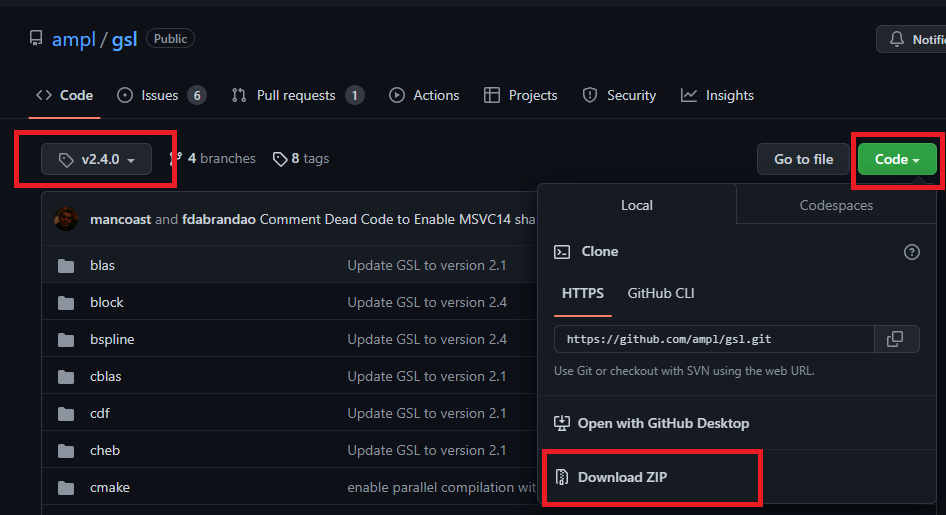
\includegraphics[width=0.9\textwidth]{../../../shared_latex_inputs/images/gsl_github.png}
		\caption{GSL Github}
	\end{figure}
	\begin{enumerate}
		\item Extract the contents of the zip file into a destination with no spaces in the file path (e.g. C:\textbackslash SW\_Installs\textbackslash gsl-2.4.0) and record its location for future use.
	\end{enumerate}
	\item \label{bundle:gsl} Open the CMake \ac{GUI}
	\item Set the CMake settings
	\begin{enumerate}
		\item Make sure that the “Advanced” and “Grouped” check boxes are checked. \\ \emph{This makes it easier to see all options}
		\item In the “Where to build the binaries:” text box, put Path/To/gsl/build. \\ It is OK if the “build” directory does not exist yet; CMake will create it. 
		\item In the “Where is the source code:” text box, put Path/To/gsl
		\item Click the ‘Configure’ button and create the build directory if prompted 
			\begin{figure}[H]
				\centering
				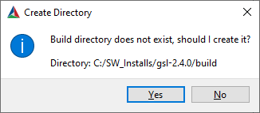
\includegraphics[width=0.5\linewidth]{../../../shared_latex_inputs/images/gsl_build_new-dir.png}
				\caption{GSL Create New Build Directory}
			\end{figure}
			\begin{figure}[H]
				\centering
				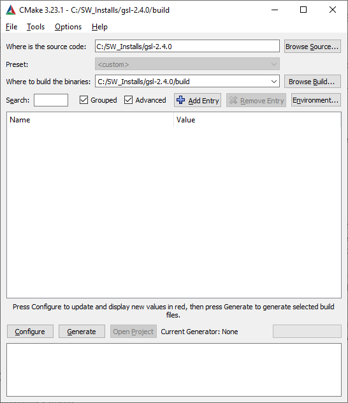
\includegraphics[width=0.7\linewidth]{../../../shared_latex_inputs/images/gsl_cmake_menu.png}
				\caption{GSL CMake Menu}
			\end{figure}
		\item If this is the first time the ‘Configure’ button has been clicked since the cache has been cleared, a popup window asking which Toolset to use will appear. Select the correct Visual Studio installation. Make sure that the “x64” toolchain is selected. \\ This pop-up can also appear on clicking the ‘Generate’ button if the cache has been cleared.
		\begin{enumerate}
			\item Verify that the “Configuring done” text is displayed in the log window
			\begin{figure}[H]
				\centering
				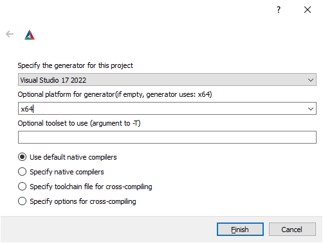
\includegraphics[width=0.7\linewidth]{../../../shared_latex_inputs/images/cmake_vstudio_select.png}
				\caption{CMake Visual Studio Settings}
			\end{figure}
		\end{enumerate}
	\end{enumerate}	
	\item Click the ‘Generate’ button
	\begin{enumerate}
		\item Verify that the “Generating done” text is displayed in the log window
	\end{enumerate}	
	\item Click the ‘Open Project’ button in the CMake GUI to open the project in Visual Studio.
	\begin{enumerate}
		\item Right-click on ‘ALL BUILD’ in the Solution Explorer pane and select the ‘Set As Startup Project’ option. 
			\begin{figure}[H]
				\centering
				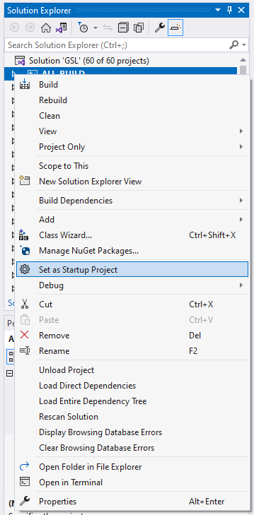
\includegraphics[width=0.35\linewidth]{../../../shared_latex_inputs/images/vstudio_set-startup.png}
				\caption{Visual Studio Select Startup Project}
			\end{figure}
		\item In the toolbar, select the ‘Release’ option from the 'Solution Configurations' dropdown.
			\begin{figure}[H]
				\centering
				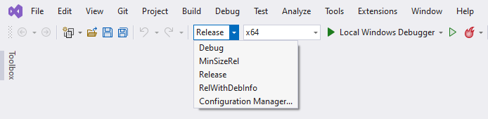
\includegraphics[width=0.7\linewidth]{../../../shared_latex_inputs/images/vstudio_config_release.png}
				\caption{Visual Studio Release Solution Configuration}
			\end{figure}
		\item Right-click on ‘ALL BUILD’ in the Solution Explorer then select the ‘Build’ option.
		\begin{enumerate}
			\item A successful build will result in a message that says, in part, “0 failed” in the Visual Studio output window. 
			\begin{figure}[H]
				\centering
				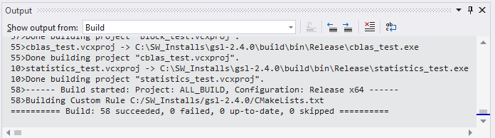
\includegraphics[width=0.7\linewidth]{../../../shared_latex_inputs/images/vstudio_gsl_success.png}
				\caption{GSL Visual Studio Success Output}
			\end{figure}
			\item The header files will be in Path/To/gsl/build/gsl.
			\item The library files will be in Path/To/gsl/build/Release.
		\end{enumerate}
	\end{enumerate}		
\end{enumerate}
